\section{Approach}
\label{sec:approach}

In this section, we describe the model architecture used for our experiments
%and propose our reducing repetition method which is implemented by extending thebasic model.
and propose our novel repetition reduction method, which is an extension to the basic model.
~\footnote{
All of the data and source code
can be downloaded from http://202.120.38.146/sumrep.}

In summarization task, the input (source document) and
output (summary) are both sequences of words.
%\XS{elements? better use words or terms}.
Suppose the input and output are respectively represented as
$\textbf{x} = (x_{1},x_{2},...,x_{m})$ and 
$\textbf{y} = (y_{1}, y_{2},..., y_{n})$ ($m>n$),
the goal is to maximize the conditional probability
$p(\textbf{y}|\textbf{x})$:
\begin{equation}
\small
p(\textbf{y} | \textbf{x}) \!=\! {\prod^T_{t} {p(y_{t} | y_{1}, y_{2},..., y_{t-1}, \textbf{x}})}
\end{equation}

%Our goal is to model the above conditional probability in such a way that the 
Furthermore, we aim to generate summaries that are not only fluent 
and logically consistent with source document, but also with 
a small amount of repeatedness, which is natural in human written summaries.  
%(results illustrated in \tabref{tab:eval_repe}). 
%We aim at getting the above conditional probability which can generate summaries without repetition.

\subsection{Basic CNN seq2seq Model}
\label{sec:basic}
Our basic model is multi-layer convolutional seq2seq networks \cite{gehring2017convs2s} with attention mechanism.
\footnote{\url{https://github.com/facebookresearch/fairseq-py}}, 
as illustrated in \figref{fig:basicModel}. 

\begin{figure}[th]
    \centering
    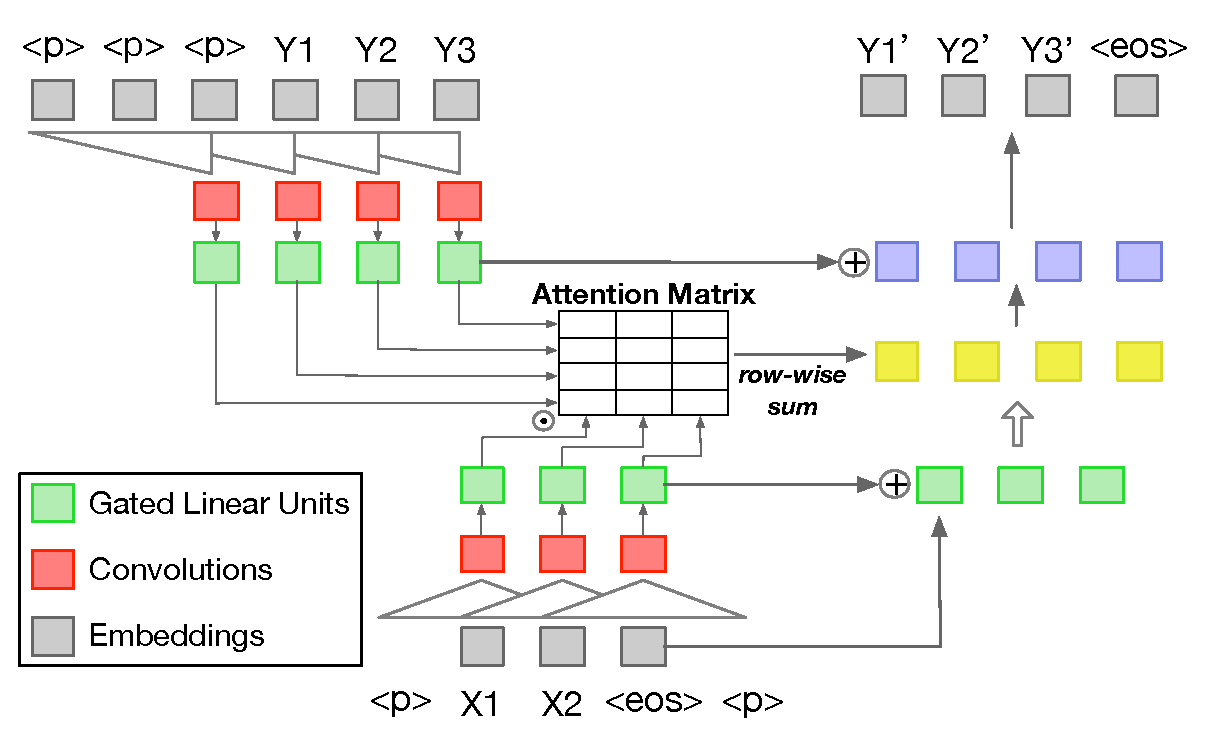
\includegraphics[width=0.8\linewidth]{cnn}
    \caption{Convolutional seq2seq model.}
	%$\odot$ stands for inner product. $\oplus$ stands for element-wise addition.}
    \label{fig:basicModel}
\end{figure}

%Our basic model includes multi-layer convolutional seq2seq networks \cite{gehring2017convs2s} and attention mechanism \footnote{\url{https://github.com/facebookresearch/fairseq-py}}, as illustrated in \figref{fig:basicModel}. 

For CNN seq2seq models, we combine both word embeddings and position embeddings to obtain input $\mathbf{X} = (X_1,...,X_m)$ and output $\mathbf{Y}=(Y_1,...,Y_n)$. 
%We denote $\mathbf { z } ^ { l }$ and $\mathbf { h } ^ { l }$ 
We denote $\mathbf { z } ^ { l } = \left( z _ { 1 } ^ { l } , \ldots , z _ { m     } ^ { l } \right)$ and $\mathbf { h } ^ { l } = \left( h _ { 1 } ^ { l } , \ldots , h _ { n } ^ { l } \right)$ 
respectively as convolutional output of the encoder and
decoder in the $l$-th layer.
%where $\mathbf { z } ^ { l } = \left( z _ { 1 } ^ { l } , \ldots , z _ { m } ^ { l } \right)$ and $\mathbf { h } ^ { l } = \left( h _ { 1 } ^ { l } , \ldots , h _ { n } ^ { l } \right)$. 
In each layer, GLU \cite{DauphinFAG17} and residual connections \cite{HeZRS16}
are used respectively as a non-linear gate and guarantee for sufficient depth of the network.  
\begin{equation}
\small
    h _ { i } ^ { l } = GLU \left( W ^ { l } \left[ h _ {i-k/2 } ^ { l - 1 } , \ldots , h _ { i+k/2 } ^ { l - 1 } \right] + b _ { w } ^ { l } \right) + h _ { i } ^ { l - 1 }
\end{equation} 
where \textit{k} is kernel width.
Next, we compute the probability distribution for the next word
using the top decoder output:
\begin{equation}
\small
    p \left( y _ { i + 1 } | y _ { 1 } , \ldots , y _ { i } , \mathbf { x } \right) = \operatorname { softmax } \left( W _ { o } h _ { i } ^ { L } + b _ { o } \right)
\end{equation}

For each decoder layer, the multi-step attention integrates encoder information. 
%We compute decoder state $d_{i}^{l}$ via
\begin{equation}
\small
    d _ { i } ^ { l } = W _ { d } ^ { l } h _ { i } ^ { l } + b _ { d } ^ { l } + Y _ { i }
\end{equation}

%The inner product between decoder state and encoder outputs is used 
%to measure the affinity. 
%The conditional input to the current 
%decoder layer is a weighted sum of encoder states and input representations.
\begin{equation}\label{eq:a}
\small
    a _ { i j } ^ { l } = \frac { \exp \left( d _ { i } ^ { l } \cdot z _ { j } ^ { u } \right) } { \sum _ { t = 1 } ^ { m } \exp \left( d _ { i } ^ { l } \cdot z _ { t } ^ { u } \right) }
\end{equation}
\begin{equation}\label{eq:c}
\small
    c _ { i } ^ { l } = \sum _ { j = 1 } ^ { m } a _ { i j } ^ { l } \left( z _ { j } ^ { u } + X_j \right)
\end{equation}
%where $z_{j}^{u}$ is the encoder output of last layer $u$.  
where $d_{i}^{l}$ is decoder state, $a_{ij}$ is attention score
and $u$ is the last layer of encoder.  
Finally, $c _ { i } ^ { l }$ is added to $h_{i}^{l}$ as the input for the next decoder layer.

\subsection{Attention Filter Mechanism (ATTF)}
\label{sec:attf}

\begin{figure}[th]
	\centering
	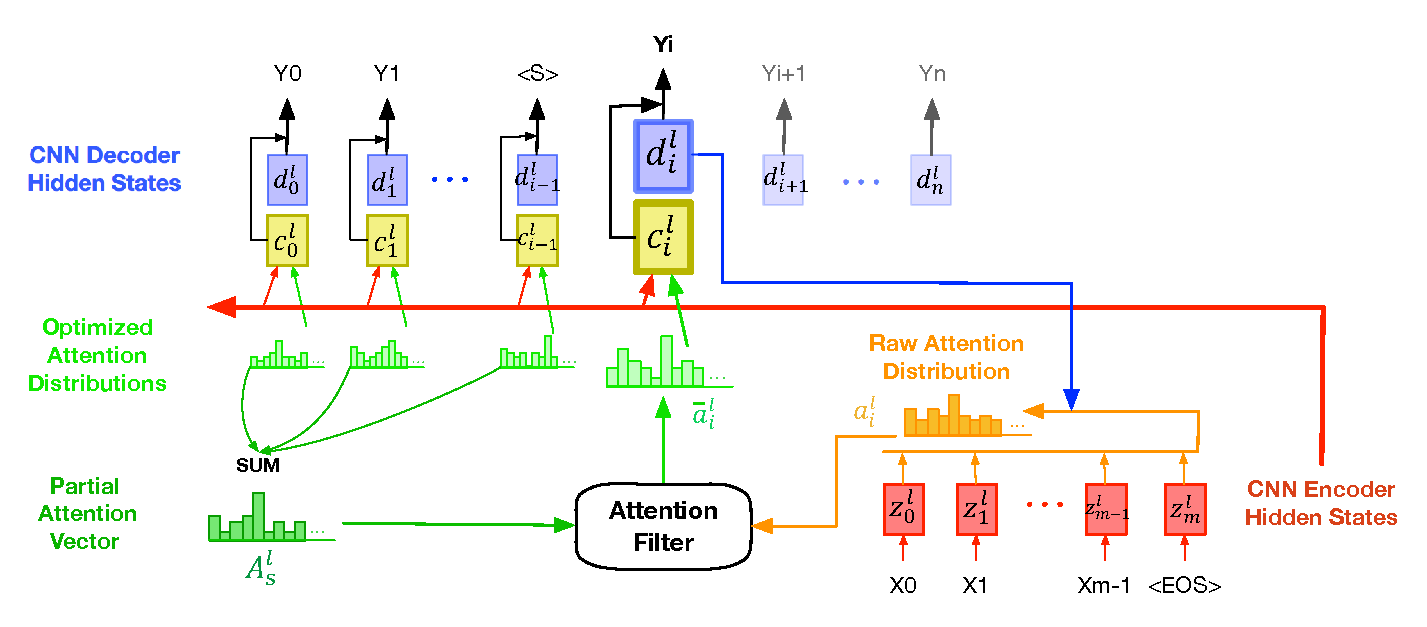
\epsfig{file=model.eps, width=1.0\columnwidth}
	%\caption{Overview of proposed model, which shows how Attention Filter Mechanism (ATTF) works when decoding $Y_i$.}
	\caption{Overview of Attention Filter Mechanism (ATTF)}
	\label{fig:model_main}
\end{figure}


\label{sec:attnf}
%We propose an attention filter mechanism based on basic model
We propose an attention filter mechanism as a novel extension 
to the basic model,
which can record previously attended locations 
%previously POIs 
in the source document directly and generate summaries 
%without repetition
with a natural level of repeatedness. 
This method aims at relieving the repetition problem caused by 
decoders attending to the same POI in source document.

In this mechanism, both source documuent and summary are 
respectively split into 
\textit{sections} and \textit{segments} by punctuations. We
denote the punctuation marks as \verb#<S>#.
$\mathbf{u}=(u_{0},u_{1},...,u_{M})$ 
and $\mathbf{v}=(v_{0},v_{1},...,v_{N})$
denote the positions of \verb#<S># in source document and summary.
Both $u_{0}$ and $v_{0}$ are $-1$.
%Source document $\mathbf{U}=(U_{0},U_{1},...,U_{M-1})$ 
%and summary $\mathbf{V}=(V_{0},V_{1},...,V_{N-1})$ are represented in the form of sections and.
Therefore, we can represent source document as $\mathbf{U}=(U_{0},U_{1},...,U_{M-1})$ in the form of \textit{sections}. Similarly, for summaries, we have $\mathbf{V}=(V_{0},V_{1},...,V_{N-1})$. 
$U_i$ and $V_i$ are
both sequence of tokens minus the punctuation tokens.
%\KW{They are all substrings splitted by punctuations.}

Let $D$ denote the number of tokens in the source document.
We define \textit{segment attention vector} in the $l$-th layer as 
$A^{l} = (A_{0}^{l}, A_{1}^{l},..., A_{N}^{l})$, 
where $A_s^l\subset \mathbb{R}^{D}$ is a vector representing 
segment attention distribution, of the $s$-th \textit{segment},
over tokens in the source document. Summing up attention score vectors 
of each position in the $s$-th \textit{segment}:
%which is the sum of attention distributions over each section in summary:

\begin{equation}
\small
    A_{s}^{l} = \sum_{i=v_{s-1}+1}^{v_{s}-1}a_{i}^{l}
\end{equation}
where $a_i^l$ is also a $D$-dimensional vector that records 
the attention scores of the $i$-th token in the summary over 
tokens in the source document. In other words, $ A_{s}^{l}$ 
measures the relevance between tokens of the source document and 
the $s$-th \textit{segment} $V_s$. 
%where vector $A_{n}^{l}$ is the partial attention distribution over the words in source document. 
%It represents the degree of relevance between source document and the $n$-th section in summary.
We set $A_{0}^{l}$ as zero vector, because nothing is attended before generating 
the first \textit{segment}. 


To find the most attended \textit{sections}, 
we sort the elements inside the filter vector, 
$A_{s}^{l}$, in descending order, 
and record the top $k$ elements' positions in 
the source document as: 
\begin{equation}
\small
    \mathbf{p}=(p_{0},...,p_{k})
\end{equation}
where $k=v_{s}-v_{s-1}-1$.
%To get the attended sections of document, we sort elements $A_{nj}^{l}$ in descending order, and record the positions a
%in decreasing order, and record the position
%$\mathbf{p}=(p_{0},...,p_{k})$, of 
%top $k$ elements in source document, where $k = v_{n} - v_{n-1}$. 
%The higher value of $A_{nj}^{l}$ means that the $j$-th words of source document has been attended. 
%We find out which section of these top $k$ elements belong to by $\mathbf{p}$ and $\mathbf{u}$.
Next, we locate these elements in the source document as well as
the \textit{sections} they belong to. 
We assign each section a set of positions that have been attended to, 
$P_{U_{t}}$. 
If the size of $P_{U_{t}}$ is larger than
$sz$, a predefined constant,
%\footnote{$sz$ is a constant. 
%We set $sz$ as 3, because nearly 90 percent
%of sections with lengt$>=$3.}, 
the \textit{section} $U_{t}$ should not be attended again. 
That is, $U_{t}$ is a POI of segment $V_{s}$.
%We use $\bar{U}$ to express this kind of section. 
$\mathbb{U}_{s}$ denotes a set of all such POIs for $V_s$.
$\mathbb{U}_{0}$ is an empty set.
%the \textit{section $U_{t}$} can be seen as the POI by $V_s^{l}$. 

We construct two multi-hot vectors $g_{s}$ and $g'_{s}$ for each \textit{segment} $V_{s}$.
The dimensions of them are the
same as $A_{s}^{l}$. For $g_{s}$, we set elements on the position of tokens
belonging to sections in $\mathbb{U}_{s}$ to 0, and other
%same as $A_{s}^{l}$. For $g_{s}$, we set elements on the position of POIs to 0, and other
positions to 1. $g'_{s}$ is the flipped version of $g_{s}$. 
The filter on $a_{ij}^{l}$ in Equation (\ref{eq:a} is to minimize elements of POIs:
%The filter on $a_{ij}^{l}$ in Equation (\ref{eq:a}) is given as:
%\KZ{Can we simplify the notations a bit? What are $A^l_{sj}$ and
%$g_{sj}'$? We had $A^l_s$ before ... It's a bit confusing.}
\begin{equation}
\small
    e_{s} = \min \limits_{A_{s}}\left(\frac{A_{sj}^{l}}{v_{s}-v_{s-1}-1}\right)
\end{equation}
\begin{equation}
\small
    \tilde{a}_{ij}^{l} = a_{ij}^{l}\prod_{q=0}^{s}g_{qj} + e_{s}g_{sj}'
    %\bar{a_{ij}}^{l} = a_{ij}^{l}\prod_{q=0}^{n}s_{q} + \min\frac{A_{n}^{l}}{v_{n}-v_{n-1}}t_{n}
\end{equation}
where $v_{s}$ is the maximum value in 
$\mathbf{v}$ that is smaller than $i$, and $\tilde{a}_{ij}^l$ is the filtered
attention score. $A_{sj}$ is the attention score between $j$-th token
of the source document and the $s$-th \textit{segment}. 
$g_{sj}$ and $g_{sj}'$ denote whether $j$-th token
of the source document has been attended.
%\XS{Hard to understand this definition of ``n''. And ``n'' is already used to be the size of output in Section 2.1}
Equation (\ref{eq:c}) now becomes:
\begin{equation}
\small
    c _ { i } ^ { l } = \sum _ { j = 1 } ^ { m } \tilde{a}_{ij}^{l} \left( z _ { j } ^ { u } + X_j \right)
\end{equation}

%We pick $K$ sections with highest attention which is calculated by:
%\begin{equation}
%    A_{nj}^{l} = \sum^{P}A_{nj}^{l}
%\end{equation}  

%This method find out the attended location in source document directly and accurately.
%Then it filters out attention of the attended location from the attention distribution. 
%%In this way, our attention filter is capable of comprehending the attention history in a precise and direct manner. 
%The previous approaches revise attention scores
%through decoder hidden state. They can not locate POIs exactly.
%The coverage model which gets the sum of all previous attention can 
%bring attention noise, especially in the long summary.

%Because of using segment attention and revising attention score of attended POIs directly,
By using segment-wise attention and revising attention score of attended POIs directly,
%it optimizes the 
%\KW{compared with token-wise attention,}
our model optimizes the
attention distribution between encoder states and decoder states in such a way that
the alignment relationship between source document and summary is enhanced, 
and noise for attention from encoder outputs is reduced. 
As shown in \tabref{tab:attn_exp}, the segments in example are separated by punctuation.
For basic CNN model, the 2nd and 3rd sentence repeatedly attend to 
the 5th segment in source.
After applying ATTF model, 
the attention score of 3rd and 5th segment in source are penalized 
during generating words in 3rd sentence of ATTF.
The last sentence of the summary generated by ATTF attend to 7th segment in source.

\begin{table}[th!]
\begin{center}
\scriptsize
\begin{tabular}{|l|l|}%{|p{7cm}|rl|}
\hline 
\multicolumn{2}{|c|}{\bf Source document} \\
\hline
\multicolumn{2}{|c|}{\tabincell{l}{(1)justin timberlake and jessica biel, (2)welcome to parenthood. 
	   (3)the celebrity couple announced the arrival \\
           of their son, 
           (4)... 
	   (5)the couple announced the pregnancy in january, (6)...  
	   (7)it is the first baby for both . }} \\
\hline 
\bf Basic CNN model (CNN) & \bf ATTF (our) \\
\hline 
\tabincell{l}{(1)the couple announced the the arrival of their son. \\
              (2)the couple announced the pregnancy in january. \\ 
              (3)the couple announced the pregnancy in january. } 
& \tabincell{l}{(1)the couple announced the arrival of their son. \\
	            (2)the couple announced the pregnancy in january. \\
	            (3)it is the first baby for both. } \\
\hline
\end{tabular}
\end{center}
\caption{\label{tab:attn_exp} Summary generated by the basic CNN model and ATTF model}
\end{table}
%The attention filter mechanism helps avoid repeatedly attending to the same POIs, and therefore avoid repetition in summary generation.


\subsection{Sentence-level Backtracking Decoder (SBD)}

%As mentioned in \secref{sec:intro}, another reason that gives rise to 
%repetition in summaries is repeated sentences or phrases in 
%source documents.
%To handle the repetition caused by repetitive sentences in source document(\tabref{tab:src_rep}),
%To tackle repeated sentences or phrases in the source document (\exref{ex:repeatsrc}), 
%we propose a sentence-level backtracking decoder at testing.
To tackle repeated sentences or phrases in the source (\exref{ex:repeatsrc}), 
we propose a sentence-level backtracking decoder.

\begin{figure}[th]
    \centering
    \includegraphics[width=0.8\linewidth]{SBD}
    \caption{Backtracking in Beam Search ($b=3$)}
    \label{fig:beam}
\end{figure}

At test time, we prevent the decoder from generating identical or
very similar sentences more than once via backtracking. 
An intuitive solution is to backtrack the generation process to the beginning
of the repeated segment, and regenerate it by following the second best choice
in the beam. We call this simple approach SBD-b1.
However, this is sub-optimal because the parents of the current top $b$
choices may not include all the top $b$ choices at the parent level, e.g.,
the first choices at level 1 and 2 are excluded by beam search,
as shown in \figref{fig:beam}. Here $b$ is the beam size.

An alternative approach (SBD-b2) backtracks all the way until the current
top $b$ choices all share the same prefix token sequence. This means
that the current best choices in the beam reach some consensus that
the generated prefix summary is good and should be retained. While
this algorithm backtracks further and may include better choices,
it doesn't completely solve the problem of SBD-b1.

Our best approach (SBD) backtracks to the beginning of the whole summary
and regenerates all the choices in the beam up to the point before
the repeated segment. That way, all the best choices are known to the
algorithm and we can make an optimal choice after excluding the first word
of the previously repeated segment. 
%When regenerating a new summary, 
%we do not generate the same word as the first word in $S$ at step $p$.
%our model do not consider the starting word of $S$ at step $p$.
%Another two versions of backtracking are compared in \secref{sec:eval}.
%One (SBD-b1) is to regenerate this sentence from the end of last sentence.
%SBD-b1 only backtracks to the beginning of the last sentence.
%The other (SBD-b2) is backtracking to the most adjust decoder state 
%that all of generated sequences in beam size
%before this state are the same.
%Whereas SBD-b2 backtracks to the timestamp where all $k$ candidate sequences in beam search are exactly the same, where $k$ denotes beam size. 
%\KW{not sure if i get it right}

To determine whether two sentences, 
$p$ and $q$, are similar, we define a boolean function as:
\begin{equation}\label{eq:s}
\small
    sim(p,q) = o > n\text{ OR }o > \frac{1}{2}\cdot l
\end{equation}
where $o$ denotes the length of the longest common substring (LCS) between $p$ and $q$, 
$l$ is the minimum of the lengths of $p$ and $q$, and $n$ is a constant. 
$sim(p,q)=1$ means the two sentence are similar.
%We set $n$ as 5, because the number of overlapped words in target summaries
%is less than 5 percent.
%\KW{maybe mention c=5 in experiment settings, the notation in the formula is not clean enough but i don't know how to revise it}

This method does not attempt to impact the process of beam search in the middle of a sentence so that we are free of grammatical and factual errors compared with our \textbf{TRI} baseline.
%This method cooperates with ATTF in 
%reducing repetition caused by the noises in the dataset.
%It does not interrupt the beam search process in the middle of a sentence, 
%hence significantly reducing related grammatical and factual errors 
%compared with \textbf{TRI}.
%which we validate in \tabref{tab:strong_methods}.
Besides, it is capable of producing a more informative summary since
it yields more chances to other candidate sentences.
%, which we validate in relevant experiments
%(\tabref{tab:src_rep}, \figref{fig:attn_map3}).
